\documentclass[@BEAMER_OPTIONS@]{beamer}
    @USE_PGFPAGES@

    \usetheme[alternativetitlepage=true,titleline=true]{Torino}
    \setbeamertemplate{navigation symbols}{}
    \setbeamertemplate{note page}[plain]
    \setbeamertemplate{caption}{\insertcaption}


    \usepackage[utf8]{inputenc}
    \usepackage[russian]{babel}
    \usepackage{graphicx}
    \usepackage{subfigure}
    \usepackage{xspace}
    \usepackage{adjustbox}
    \usepackage{tikz}
    \usepackage{relsize}
    \usepackage{fancyvrb}
    \fvset{fontsize=\footnotesize}
    \RecustomVerbatimEnvironment{verbatim}{Verbatim}{}
    \usepgflibrary{arrows}
    \usetikzlibrary{shadows,decorations.pathreplacing,patterns,shapes}
    \tikzstyle{every picture}=[semithick,>=stealth,remember picture]
    \usepackage{inconsolata}
    \usepackage{listings}
    \lstset{
        language=C++,
        basicstyle=\footnotesize\rmfamily,
        keywordstyle=\color{chameleon4}\bfseries,
        commentstyle=\color{chameleon1}\it\rmfamily,
        stringstyle=\color{chameleon4},
        numbers=left,
        numberstyle=\tiny,
        aboveskip=-0.02\baselineskip,
        belowskip=-0.02\baselineskip,
        columns=flexible,
        extendedchars=false,
        showstringspaces=false,
        morekeywords={global,kernel,ulong,size_t,cl_uint,cl_platform_id}
        }
    \newcommand{\code}[1]{\lstinline|#1|}
    \protected\def\plusplus{{\nolinebreak[4]\hspace{-.05em}\raisebox{.4ex}{\relsize{-3}\bf ++}}\xspace}
    \newcommand{\CXX}{{\rm C}\plusplus}
    \newcommand{\CC}{{\rm C99}\xspace}
    \newcommand{\www}[1]{\href{#1}{#1}}

    \usepackage{ifthen}
\usetikzlibrary{shadows.blur}
\newlength{\ribbonoffset}
\setlength{\ribbonoffset}{3em}

% corner, color, text
\newcommand{\ribbon}[3]{
  \ifthenelse{\equal{#1}{east}}{%
    \tikzset{ribbonrot/.style={rotate=-45}}
  }{%
    \tikzset{ribbonrot/.style={rotate=45}}
  }
  \begin{tikzpicture}[remember picture, overlay]
    \node[ribbonrot, shift={(0, -\ribbonoffset)}] at (current page.north #1) {
      \begin{tikzpicture}[remember picture, overlay,scale=0.5]
        \node[
            fill=#2,
            text centered,
            minimum width=50em,
            minimum height=1.2em,
            blur shadow,
            shadow yshift=0pt,
            shadow xshift=0pt,
            shadow blur radius=.2em,
            shadow opacity=50,
            text=white
            ](fmogh) at (0pt, 0pt) {%
            \fontfamily{phv}\selectfont\bfseries\tiny#3};
        \draw[
            white,
            dashed,
            line width=.04em,
            dash pattern=on .2em off 1.5\pgflinewidth
            ] (-25em,1em) rectangle (25em,-1em);
      \end{tikzpicture}
    };
  \end{tikzpicture}
}

    \newcommand{\forkme}{\ribbon{east}{chameleon1}{chameleon2}{\href{https://github.com/ddemidov/vexcl}{Fork me on GitHub}}}
    %\newcommand{\singledevice}{\ribbon{east}{chameleon2}{chameleon4}{Одно устройство}}
    \newcommand{\singledevice}{}

    \tikzset{
        treenode/.style={
            draw,
            fill=white,
            blur shadow,
            shadow xshift=1pt,
            shadow yshift=-1pt,
            shadow blur radius=2pt,
            shadow opacity=40
            }
        }


    \title{VexCL}
    \subtitle{Библиотека векторных выражений для GPGPU}
    \author{Денис Демидов}
    \institute{
        Градиент Технолоджи,\\
        Институт системных исследований РАН
    }
    \date{24.01.2017}

\begin{document}

%----------------------------------------------------------------------------
\begin{frame}{}
    \titlepage
\end{frame}

%----------------------------------------------------------------------------
\section{Введение}

\begin{frame}{VexCL~--- библиотека векторных выражений для OpenCL/CUDA}
    \forkme
    \begin{itemize}
        \item Создана для облегчения разработки GPGPU приложений на \CXX
            \begin{itemize}
                \item Удобная нотация для векторных выражений
                \item Автоматическая генерация вычислительных ядер во время
                    выполнения
            \end{itemize}
            \vspace{\baselineskip}
        \item Поддерживаемые технологии
            \begin{itemize}
                \item OpenCL (Khronos \CXX API, Boost.Compute)
                \item NVIDIA CUDA
                \item OpenMP
            \end{itemize}
            \vspace{\baselineskip}
        \item Исходный код доступен под лицензией MIT
            \begin{itemize}
                \item \www{https://github.com/ddemidov/vexcl}
            \end{itemize}
    \end{itemize}
\end{frame}

\note[itemize]{
\item VexCL is a vector expression template library for OpenCL. It allows you
    to use convenient matlab-like notation for vector operations and it
    generates the appropriate compute kernels for you automatically.
\item The library is header-only, so you don't have to build it to use it. The
    source code of the library is available on GitHub under very liberal
    MIT license.
}

%----------------------------------------------------------------------------
\begin{frame}{Реализация: шаблоны выражений}
    \begin{itemize}
        \item Как эффективно реализовать предметно-ориентированный язык в \CXX?
            \vspace{\baselineskip}
        \item Основная идея не нова:
            \begin{description}[Сегодня:]
                \item[1995:] \emph{Todd Veldhuizen}, Expression templates,
                    \CXX Report.
                \item[1996:]
                    Blitz{\raisebox{.2ex}{\relsize{-3}\bf ++}}\xspace:
                    библиотека \CXX для научных расчетов,\\
                    \emph{сравнимая по произодительности с Фортраном 77/90}.
                \item[Сегодня:] Armadillo, Blaze, Boost.uBLAS, Eigen, MTL,
                    и~т.~д.
            \end{description}
            \vspace{\baselineskip}
        \item VexCL использует этот подход для автоматической генерации\\
            вычислительных ядер OpenCL/CUDA
    \end{itemize}
\end{frame}

\note{ }

%----------------------------------------------------------------------------
\begin{frame}[fragile]{Hello VexCL: сложение векторов}
    \vspace{-1\baselineskip}
    \begin{columns}
        \begin{column}{0.7\textwidth}
            \begin{minipage}[c][\textheight][c]{\linewidth}
                \begin{exampleblock}{VexCL}
                    \begin{adjustbox}{width=0.7\textwidth, height=\textheight, keepaspectratio}
                        \begin{minipage}{\textwidth}
                            \lstinputlisting[linerange={1-19}]{code/hello-vexcl.cpp}
                        \end{minipage}
                    \end{adjustbox}
                \end{exampleblock}
            \end{minipage}
        \end{column}
        \begin{column}{0.25\textwidth}
            \begin{minipage}[c][\textheight][c]{\linewidth}
                \begin{exampleblock}{OpenCL}
                    \begin{adjustbox}{width=0.24\textwidth, height=\textheight, keepaspectratio}
                        \begin{minipage}{\textwidth}
                            \lstinputlisting[linerange={1-72}]{code/hello-opencl.cpp}
                        \end{minipage}
                    \end{adjustbox}
                \end{exampleblock}
            \end{minipage}
        \end{column}
    \end{columns}
\end{frame}

\note[itemize]{
\item Here is the simplest example of using vexcl: addition of two vectors on a
    gpu card.
\item The first line is the context initialization. We provide a device filter
    to the context constructor and get all compute devices that satisfy the
    filter. Here we filter by type and get all available GPUs.
\item Data allocation and transfer is also simplified. \code{vex::vector}
    constructor allocates memory on device and possibly transfers initial data
    as well. The parameters here are list of command queues and either size or
    input host vector.
\item Line ten does what's needs to be done here. This simple expression leads
    to automatic kernel generation and launch. And then we copy the results
    back to host and see what we got.
}

%----------------------------------------------------------------------------
\section{Интерфейс}

\begin{frame}
    \sectionpage
\end{frame}

%----------------------------------------------------------------------------
\begin{frame}[fragile]{Инициализация}
    \begin{itemize}
        \item Поддерживается одновременная работа с несколькими устройствами.
        \item Контекст VexCL получает \emph{фильтр устройств} при
            инициализации.
    \end{itemize}
    \begin{overlayarea}{\textwidth}{0.4\textheight}
    \begin{exampleblock}{Инициализируем контекст VexCL на выбранных устройствах}
        \begin{onlyenv}<1>
        \begin{lstlisting}
vex::Context ctx( vex::Filter::Any );
        \end{lstlisting}
        \end{onlyenv}
        \begin{onlyenv}<2|handout:0>
        \begin{lstlisting}
vex::Context ctx( vex::Filter::GPU );
        \end{lstlisting}
        \end{onlyenv}
        \begin{onlyenv}<3|handout:0>
        \begin{lstlisting}
vex::Context ctx(vex::Filter::Accelerator && vex::Filter::Platform("Intel"));
        \end{lstlisting}
        \end{onlyenv}
    \end{exampleblock}
    \end{overlayarea}
    \begin{figure}
        \uncover<1-2>{
            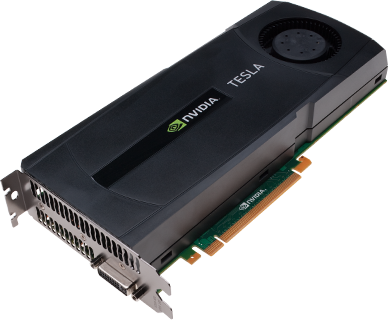
\includegraphics[width=0.2\textwidth]{tesla.png}\quad
        }
        \uncover<1,2>{
            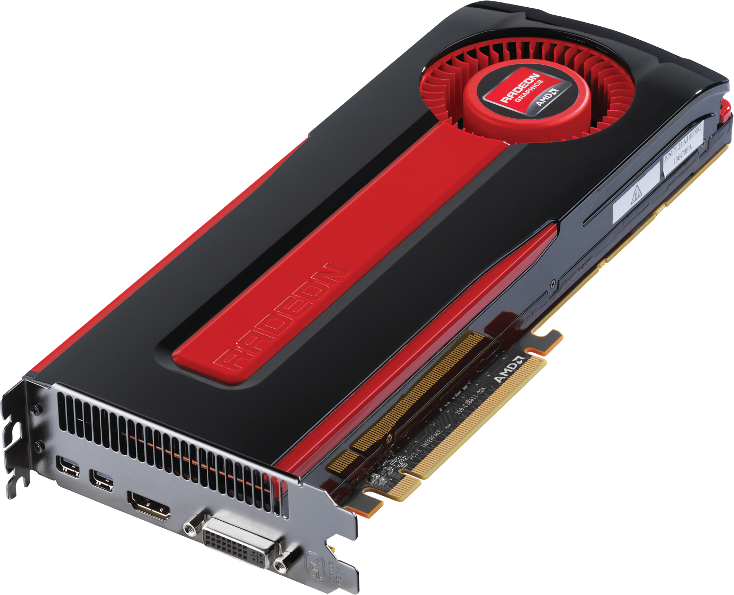
\includegraphics[width=0.2\textwidth]{radeon.png}\quad
        }
        \uncover<1,3>{
            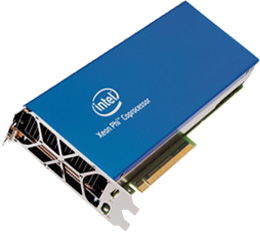
\includegraphics[width=0.17\textwidth]{intel.png}
        }
    \end{figure}
\end{frame}

\note[itemize]{
\item VexCL can transparently work with several compute devices that are
    present on your system.
\item We initialize the VexCL context with a device filter. The device filter
    is a simple functor that acts on device reference and returns a boolean
    value. Several standard filters are provided and you can write your own
    filters.
\item Let's assume that we have an NVIDIA GPU, an AMD GPU, and an Intel CPU
    installed.
    \begin{enumerate}
        \item The standard 'All' Filter select any device available, so we end
            with three devices in our context.
        \item If we want to select only GPUs, then we can filter the devices by
            type.
        \item It is also possible to combine the device filters with logical
            operators.  Here we select a GPU that is provided by AMD OpenCL
            platform.
        \item And here is an example of a custom filter. Here it selects any
            device that has at least 4GB of memory.
    \end{enumerate}
}

%----------------------------------------------------------------------------
\begin{frame}[fragile]{Распределение памяти и вычислений между картами}
    \setbeamercovered{transparent=40}
    \begin{exampleblock}{}
        \begin{onlyenv}<1|handout:0>
        \begin{lstlisting}
vex::Context ctx( vex::Filter::Name("Tesla") );
        \end{lstlisting}
        \end{onlyenv}
        \begin{onlyenv}<2|handout:0>
        \begin{lstlisting}
vex::Context ctx( vex::Filter::Type(CL_DEVICE_TYPE_GPU) );
        \end{lstlisting}
        \end{onlyenv}
        \begin{onlyenv}<3>
        \begin{lstlisting}
vex::Context ctx( vex::Filter::DoublePrecision );
        \end{lstlisting}
        \end{onlyenv}
        \begin{uncoverenv}<1>
        \begin{lstlisting}[firstnumber=last]

vex::vector<double> x(ctx, N);
vex::vector<double> y(ctx, N);

x = vex::element_index() * (1.0 / N);
y = sin(2 * x) + sqrt(1 - x * x);
        \end{lstlisting}
        \end{uncoverenv}
    \end{exampleblock}
    \setbeamercovered{invisible}
    \begin{figure}
        \begin{tikzpicture}
            \draw (0,2.5) rectangle +(8,0.1);
            \draw (0,2.5) grid[step=0.1] +(8,0.1);
            \draw (-0.3,2.6) node{x};

            \draw (0,2.0) rectangle +(8,0.1);
            \draw (0,2.0) grid[step=0.1] +(8,0.1);
            \draw (-0.3,2.1) node[anchor=center]{y};

            \uncover<1-3> {
            \draw (1,0.5) node{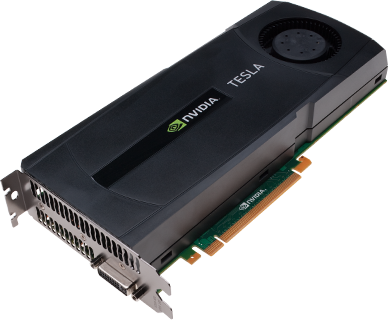
\includegraphics[width=0.2\textwidth]{tesla.png}};
            }

            \uncover<2-3> {
            \draw (4,0.5) node{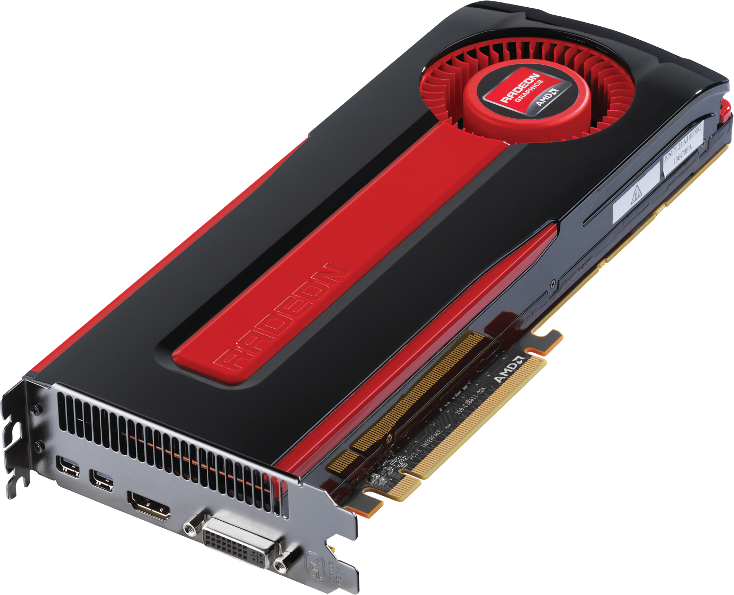
\includegraphics[width=0.2\textwidth]{radeon.png}};
            }

            \uncover<3> {
            \draw (7.5,0.5) node{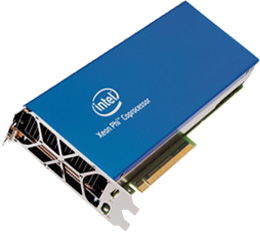
\includegraphics[width=0.17\textwidth]{intel.png}};
            }

            \uncover<1|handout:0> {
            \draw[->,chameleon1,style=dashed] (0,2.7) -- (0,1.8)
                .. controls +(east:0.5) and +(north west:0.5) ..
                (1.4,1.5);
            \draw[->,chameleon1,style=dashed] (8,2.7) -- (8,1.8)
                .. controls +(west:0.5) and +(north east:0.5) ..
                (1.6,1.5);
            }

            \uncover<2|handout:0> {
            \draw[->,chameleon1,style=dashed] (0,2.7) -- (0,1.8)
                .. controls +(east:0.5) and +(north west:0.5) ..
                (1.4,1.5);
            \draw[->,chameleon1,style=dashed] (4,2.7) -- (4,1.8)
                .. controls +(west:0.5) and +(north east:0.5) ..
                (1.6,1.5);

            \draw[->,chameleon1,style=dashed] (4,2.7) -- (4,1.8)
                .. controls +(east:0.1) and +(north west:0.2) ..
                (4.4,1.5);
            \draw[->,chameleon1,style=dashed] (8,2.7) -- (8,1.8)
                .. controls +(west:0.5) and +(north east:0.5) ..
                (4.6,1.5);
            }

            \uncover<3> {
            \draw[->,chameleon1,style=dashed] (0,2.7) -- (0,1.8)
                .. controls +(east:0.5) and +(north west:0.5) ..
                (1.4,1.5);
            \draw[->,chameleon1,style=dashed] (3,2.7) -- (3,1.8)
                .. controls +(west:0.5) and +(north east:0.5) ..
                (1.6,1.5);

            \draw[->,chameleon1,style=dashed] (3,2.7) -- (3,1.8)
                .. controls +(east:0.5) and +(north west:0.2) ..
                (4.4,1.5);
            \draw[->,chameleon1,style=dashed] (6,2.7) -- (6,1.8)
                .. controls +(west:0.5) and +(north east:0.5) ..
                (4.6,1.5);

            \draw[->,chameleon1,style=dashed] (6,2.7) -- (6,1.8) -- (7.4,1.5);
            \draw[->,chameleon1,style=dashed] (8,2.7) -- (8,1.8) -- (7.6,1.5);
            }
        \end{tikzpicture}
    \end{figure}
\end{frame}

\note[itemize]{
\item Now that we know how to initialize VexCL context, let's see how device
    vectors are allocated.
\item Here we allocate three vectors, and initialize two of them with
    constant values.
\item Each vector receives a list of queues at initialization.  Since each
    queue corresponds to a specific device, vectors know where to put their
    data to.
    \begin{enumerate}
        \item For example, if we only have the Tesla card in our context, then
            it will hold the complete memory for all of our vectors.
        \item If we use both of the available GPUs, then the vectors will be
            split between the devices. This split is by default proportional to
            the GPU bandwidth and is guaranteed to be consistent for vectors of
            the same size. This consistency allows VexCL to run computations
            independently on all devices in context.
        \item If we add the CPU to the context, it will get smaller share of
            the data and arithmetic operations.
    \end{enumerate}
\item Care must be taken with the use of several devices. VexCL tries to split
    the memory as fair as it can, but it is probable that your program will
    run at the speed of the slowest device.
}

%----------------------------------------------------------------------------
\begin{frame}[fragile]{Язык векторных выражений VexCL}
    \begin{itemize}
        \item Все векторы в выражении должны быть \emph{совместимыми}:
            \begin{itemize}
                \item Иметь один размер
                \item Быть расположенными на одних и тех же устройствах
            \end{itemize}
        \item Что можно использовать в выражениях:
            \begin{columns}
                \begin{column}{0.4\textwidth}
                    \begin{itemize}
                        \item Векторы, скаляры, константы
                        \item Арифм. и логич. операторы
                        \item Встроенные функции
                        \item Пользовательские функции
                        \item Генераторы случайных чисел
                        \item Сортировка, префиксные суммы
                    \end{itemize}
                \end{column}
                \begin{column}{0.4\textwidth}
                    \begin{itemize}
                        \item Временные значения
                        \item Срезы и перестановки
                        \item Редукция (сумма, экстремумы)
                        \item Произв. матрицы на вектор
                        \item Свертки
                        \item Быстрое преобразование Фурье
                    \end{itemize}
                \end{column}
            \end{columns}
    \end{itemize}
\end{frame}

\note[itemize]{
\item So, what kind of expressions can you use in VexCL?
\item First, any vectors used in an expression have to be compatible.
\item If this requirement is satisfied, then expressions may combine
    vectors and scalars with almost any binary operators. OpenCL math functions
    and user-defined functions are also available.
}

%----------------------------------------------------------------------------
\begin{frame}[fragile]{Встроенные операторы и функции}
    \begin{columns}
        \begin{column}{0.38\textwidth}
            \begin{exampleblock}{Выражение:}
                \begin{lstlisting}
x = 2 * y - sin(z);
                \end{lstlisting}
            \end{exampleblock}
        \end{column}
        \begin{column}{0.55\textwidth}
            \begin{itemize}
                \item \code{export VEXCL_SHOW_KERNELS=1}\\
                    чтобы увидеть сгенерированный код.
            \end{itemize}
        \end{column}
    \end{columns}
    \begin{exampleblock}{\ldots генерирует ядро:}
        \begin{lstlisting}
kernel void vexcl_vector_kernel(
    ulong n,
    global double * prm_1,
    int prm_2,
    global double * prm_3,
    global double * prm_4
)
{
    for(size_t idx = get_global_id(0); idx < n; idx += get_global_size(0)) {
        prm_1[idx] = ( ( prm_2 * prm_3[idx] ) - sin( prm_4[idx] ) );
    }
}
        \end{lstlisting}
    \end{exampleblock}
    \begin{tikzpicture}[overlay,scale=0.6]
        \draw (16,8) node(sub)[draw,fill=white,ellipse,drop shadow]{$-$};

        \draw (sub) +(-2.00,-1) node(mul)[draw,fill=white,drop shadow,ellipse]{$*$};
        \draw (sub) +( 2.00,-1) node(sin)[draw,fill=white,drop shadow,ellipse]{sin};
        \draw (mul) +(-2.00,-1) node(two)[draw,fill=white,drop shadow,minimum size=0.5cm]{2};
        \draw (mul) +( 2.00,-1) node(y)  [draw,fill=white,drop shadow,minimum size=0.5cm]{y};
        \draw (sin) +( 1.75,-1) node(z)  [draw,fill=white,drop shadow,minimum size=0.5cm]{z};

        \draw (sub) -- (mul);
        \draw (sub) -- (sin);
        \draw (mul) -- (two);
        \draw (mul) -- (y);
        \draw (sin) -- (z);
    \end{tikzpicture}
\end{frame}

%----------------------------------------------------------------------------
\begin{frame}[fragile]{Индексы элементов}
    \begin{itemize}
        \item \code{vex::element_index(size_t offset = 0, size_t size = 0)}\\
            возвращает индекс текущего элемента вектора.
            \begin{itemize}
                \item Нумерация начинается с \code{offset}, элементы на всех
                    устройствах нумеруются последовательно.
                \item Необязательный параметр \code{size} задает размер
                    выражения.
            \end{itemize}
    \end{itemize}
    \begin{exampleblock}{Линейная функция:}
        \begin{lstlisting}
vex::vector<double> X(ctx, N);
double x0 = 0, dx = 1e-3;
X = x0 + dx * vex::element_index();
        \end{lstlisting}
    \end{exampleblock}
    \begin{exampleblock}{Один период функции синуса:}
        \begin{lstlisting}
X = sin(2 * M_PI / N * vex::element_index());
        \end{lstlisting}
    \end{exampleblock}
\end{frame}

\note[itemize]{
\item \code{element_index} is a function that allows you to use element
    position inside of vector expressions.
\item The function may participate in arbitrary vector expressions.
\item For example, here\ldots
}

%----------------------------------------------------------------------------
\begin{frame}[fragile]{Пользовательские функции}
    \begin{exampleblock}{Определение функции:}
        \begin{lstlisting}
VEX_FUNCTION( double, sqr, (double, x)(double, y),
    return x * x + y * y;
    );
        \end{lstlisting}
    \end{exampleblock}
    \begin{exampleblock}{Использование функции:}
        \begin{lstlisting}
Z = sqrt( sqr(X, Y) );
        \end{lstlisting}
    \end{exampleblock}
\end{frame}

\note[itemize]{
\item It is possible to define an OpenCL function that may be used with vector
    expressions. You need to provide function body, parameter types, and return
    type.
\item Function body has to be of \code{extern const char} type, to allow its
    use as a template parameter. And it has to be defined at global scope.
\item Inside the body function parameters are always named prm1, prm2, etc.
\item Here we define 'between' function that returns true if its second
    parameter is between its first and third parameters. The UserFunction
    object is stateless, so it may be good idea to define it at global scope
    as well, next to its body.
\item Now we may use the function in expressions. Any vector expression may be
    used as a parameter for a user-defined (or builtin) function.
}

%----------------------------------------------------------------------------
\begin{frame}[fragile]{Пользовательские функции транслируются в функции OpenCL}
    \begin{exampleblock}{}
        \begin{lstlisting}
Z = sqrt( sqr(X, Y) );
        \end{lstlisting}
    \end{exampleblock}
    \begin{exampleblock}{\ldots ведет к генерации ядра:}
        \begin{lstlisting}
double sqr(double x, double y) {
    return x * x + y * y;
}

kernel void vexcl_vector_kernel(
    ulong n,
    global double * prm_1,
    global double * prm_2,
    global double * prm_3
)
{
    for(size_t idx = get_global_id(0); idx < n; idx += get_global_size(0)) {
        prm_1[idx] = sqrt( sqr( prm_2[idx], prm_3[idx] ) );
    }
}
        \end{lstlisting}
    \end{exampleblock}
\end{frame}

%----------------------------------------------------------------------------
\begin{frame}[fragile]{Генерация случайных чисел}
    \begin{itemize}
        \item В VexCL реализованы позиционные генераторы случайных
            чисел\footnote{Random123 suite, D. E. Shaw Research,
            \href{http://www.deshawresearch.com/resources\_random123.html}{deshawresearch.com/resources\_random123.html}}
            (counter-based random number generators).
            \begin{itemize}
                \item Такие генераторы не имеют состояния и позволяют\\
                    получить случайное число по его номеру (позиции) за O(1).
                \item Реализованные семейства: \code{threefry} и \code{philox}.
                \item Удовлетворяют тестам TestU01/BigCrush; позволяют
                    получить\\ до \alert{$2^{64}$} независимых
                    последовательностей с периодом \alert{$2^{128}$}.
                \item Производительность: \alert{$\approx
                    2\times10^{10}$}~чисел/сек (Tesla K40c).
            \end{itemize}
        \item \code{vex::Random<T, G=philox>}~--- равномерное распределение.
        \item \code{vex::RandomNormal<T, G=philox>}~--- нормальное распределение.
    \end{itemize}
    \begin{exampleblock}{}
        \begin{lstlisting}
vex::Random<double> rnd;
vex::vector<double> x(ctx, n);

x = rnd(vex::element_index(), std::rand());
        \end{lstlisting}
    \end{exampleblock}
\end{frame}

\note[itemize]{
\item Random number generation is a useful feature that is used often in, e.g.,
    molecular dynamics.
\item Random number generators in VexCL are stateless, so they don't require
    additional storage or global memory interactions. Randomness is obtained by
    applying mixing functions to element indices.
}

%----------------------------------------------------------------------------
\begin{frame}[fragile]{Редукция}
    \begin{itemize}
        \item Класс \code{vex::Reductor<T, kind=SUM>} позволяет редуцировать
            произвольное \emph{векторное выражение} и получить значение типа
            \code{T}.
        \item Виды редукции: \code{SUM}, \code{SUM_Kahan}, \code{MIN},
            \code{MAX}
    \end{itemize}
    \begin{exampleblock}{Скалярное произведение}
        \begin{lstlisting}
vex::Reductor<double> sum(ctx);
double s = sum(x * y);
        \end{lstlisting}
    \end{exampleblock}
    \begin{exampleblock}{Число элементов в интервале (0, 1)}
        \begin{lstlisting}
vex::Reductor<size_t> sum(ctx);
size_t n = sum( (x > 0) && (x < 1) );
        \end{lstlisting}
    \end{exampleblock}
    \begin{exampleblock}{Максимальное расстояние от центра}
        \begin{lstlisting}
vex::Reductor<double, vex::MAX> max(ctx);
double d = max( sqrt(x * x + y * y) );
        \end{lstlisting}
    \end{exampleblock}
\end{frame}

\note[itemize]{
\item Reduction is an operation of reducing a vector to a single value.
\item The most frequent types are summation and finding minimum or maximum
    element of a vector.
\item VexCL provides Reductor functor that accepts any valid vector expression
    as a parameter.
\item For example, to compute an inner product of two vectors we compute sum of
    their elementwise product.
\item To find number of elements in vector x that are greater than zero and
    less than one, we compute sum of the corresponding boolean expression.
\item And to find the maximum distance from axis origin for a set of
    two-dimensional points, we compute exactly that: max of their radius.
}

%----------------------------------------------------------------------------
\begin{frame}[fragile]{Пример: число $\pi$ методом Монте-Карло}
    \vspace{-1\baselineskip}
    \begin{columns}
        \begin{column}{0.55\textwidth}
            \begin{itemize}
                \item Приближенная оценка $\pi$:
            \end{itemize}
            \vspace{\baselineskip}
            \begin{equation*}
                \frac{\text{площадь круга}}{\text{площадь квадрата}} =
                \frac{\pi r^2}{(2r)^2} = \frac{\pi}{4},
            \end{equation*}
            \begin{equation*}
                \pi = 4 \frac{\text{площадь круга}}{\text{площадь квадрата}}
                \approx 4 \frac{\text{\color{chameleon1}{точки в
                круге}}}{\text{\color{chameleon4}{все}
                \color{chameleon1}{точки}}}
            \end{equation*}
        \end{column}
        \begin{column}{0.35\textwidth}
            \begin{figure}
                \includegraphics[width=\textwidth]{mcpi}
            \end{figure}
        \end{column}
    \end{columns}
    \begin{exampleblock}{}
        \begin{lstlisting}[texcl=true]
vex::Random<cl_double2> rnd;
vex::Reductor<size_t, vex::SUM> sum(ctx);

double pi = 4.0 * sum( length( rnd(vex::element_index(0, n), seed) ) < 1 ) / n;
        \end{lstlisting}
    \end{exampleblock}
\end{frame}

\note[itemize]{
\item Here is a bit more complex example of what you can do with VexCL.
\item Imagine we want to compute an approximate value of $\pi$ with Monte-Carlo
    method. We can use the following equalities to do this.
}

%----------------------------------------------------------------------------
\begin{frame}[fragile]{Монте-Карло $\pi$: сгенерированное ядро}
    \begin{columns}
        \begin{column}[t]{0.2\textwidth}
            \begin{exampleblock}{}
                \begin{adjustbox}{width=0.23\textwidth, height=\textheight, keepaspectratio}
                    \begin{minipage}{\textwidth}
                        \lstinputlisting[linerange={1-49}]{code/pi-kernel.cpp}
                    \end{minipage}
                \end{adjustbox}
            \end{exampleblock}
        \end{column}
        \begin{column}[t]{0.2\textwidth}
            \begin{exampleblock}{}
                \begin{adjustbox}{width=0.23\textwidth, height=\textheight, keepaspectratio}
                    \begin{minipage}{\textwidth}
                        \lstinputlisting[firstnumber=last,linerange={50-98}]{code/pi-kernel.cpp}
                    \end{minipage}
                \end{adjustbox}
            \end{exampleblock}
        \end{column}
        \begin{column}[t]{0.2\textwidth}
            \begin{exampleblock}{}
                \begin{adjustbox}{width=0.23\textwidth, height=\textheight, keepaspectratio}
                    \begin{minipage}{\textwidth}
                        \lstinputlisting[firstnumber=last,linerange={99-147}]{code/pi-kernel.cpp}
                    \end{minipage}
                \end{adjustbox}
            \end{exampleblock}
        \end{column}
        \begin{column}[t]{0.3\textwidth}
            \begin{exampleblock}{}
                \begin{adjustbox}{width=0.23\textwidth, height=\textheight, keepaspectratio}
                    \begin{minipage}{\textwidth}
                        \lstinputlisting[firstnumber=last,linerange={148-196}]{code/pi-kernel.cpp}
                        \vspace{\baselineskip}
                    \end{minipage}
                \end{adjustbox}
            \end{exampleblock}
        \end{column}
    \end{columns}
\end{frame}

%----------------------------------------------------------------------------
\section{Оценка производительности}

\begin{frame}
    \sectionpage
\end{frame}

%----------------------------------------------------------------------------
\begin{frame}[fragile]{Параметрическое исследование системы Лоренца}
    \begin{columns}
        \begin{column}{0.6\textwidth}
            \begin{block}{Система Лоренца}
                \vspace{-1\baselineskip}
                \begin{align*}
                    \dot{x} &= -\sigma \left( x - y \right), \\
                    \dot{y} &= R x - y - xz, \\
                    \dot{z} &= -bz + xy.
                    \label{eq:lorenz}
                \end{align*}
            \end{block}
            \begin{itemize}
                \item Необходимо решать большое число систем Лоренца
                    для различных значений $R$.
                \item Будем использовать Boost.odeint.
            \end{itemize}
        \end{column}
        \begin{column}{0.4\textwidth}
            \begin{figure}
                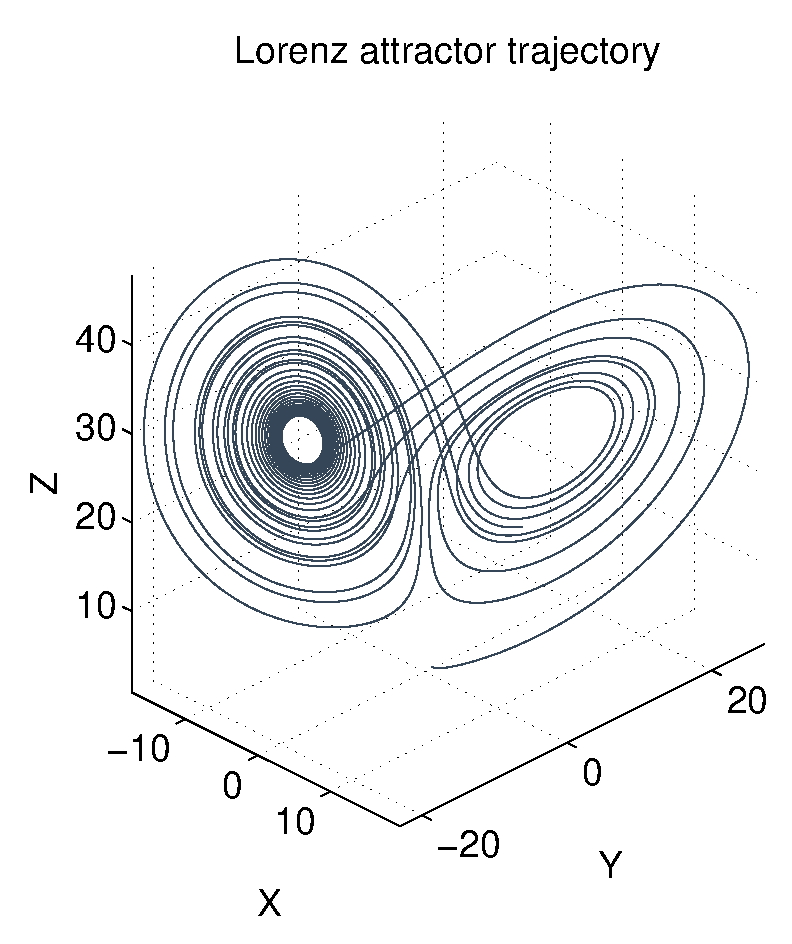
\includegraphics[width=\textwidth]{lorenz}
            \end{figure}
        \end{column}
    \end{columns}
\end{frame}

\note[itemize]{
\item As an example, lets solve a Lorenz attractor system of ordinary
    differential equations.
\item Lorenz attractor is a particle that moves according to these governing
    equations. The plot on the right shows an example of particle trajectory in
    time.
\item We will solve large number of these Lorenz systems at once.  Each of the
    systems will have its own value for parameter R. That's why this is called
    a parameter study.
}

%----------------------------------------------------------------------------
\begin{frame}{Boost.odeint}{Библиотека алгоритмов для интегрирования ОДУ}
    \begin{block}{Общий вид ОДУ}
        \begin{equation*}
            \frac{\mbox{d} x}{\mbox{d} t } = \dot{x} = f(x , t),
            \quad \quad x(0) = x_0.
        \end{equation*}
    \end{block}

    \vspace{\baselineskip}

    \begin{exampleblock}{Применение Boost.odeint:}
        \begin{enumerate}
            \item Определяем тип переменной состояния (что такое $x$?)
            \item Определяем системную функцию ($f$)
            \item Выбираем алгоритм интегрирования
            \item Выполняем интегрирование по времени
        \end{enumerate}
    \end{exampleblock}
\end{frame}

\note[itemize]{
\item Here is a general form of an ODE.
\item In order to use Boost.odeint, one has to...
}

%----------------------------------------------------------------------------
\begin{frame}[fragile]{Простейшая реализация с VexCL}
    \begin{exampleblock}{1. Тип переменной состояния}
        \begin{lstlisting}
typedef vex::multivector<double, 3> state_type;
        \end{lstlisting}
    \end{exampleblock}

    \begin{exampleblock}{2. Системная функция}
        \begin{lstlisting}[firstnumber=last]
struct lorenz_system {
    const vex::vector<double> &R;

    void operator()(const state_type &x, state_type &dxdt, double t) {
        dxdt = std::tie( sigma * ( x(1) - x(0) ),
                         R * x(0) - x(1) - x(0) * x(2),
                         x(0) * x(1) - b * x(2)  );
    }
};
        \end{lstlisting}
    \end{exampleblock}
\end{frame}

\note[itemize]{
\item We will hold current state of the system (or set of attractor
    coordinates) in a multivector with 3 components.
\item Here is the definition of the Lorenz system functor: It computes the time
    derivative from current state and time (which is not used here).
\item VexCL make the definition of the functor very simple and intuitive: we
    assign a tuple of vector expressions to the multivector that represents
    time derivative.
}

%----------------------------------------------------------------------------
\begin{frame}[fragile]{}
    \begin{exampleblock}{3. Алгоритм (Рунге-Кутты 4-го порядка)}
        \begin{lstlisting}[firstnumber=last]
odeint::runge_kutta4<
        state_type /*state*/,      double /*value*/,
        state_type /*derivative*/, double /*time*/,
        odeint::vector_space_algebra, odeint::default_operations
        > stepper;
        \end{lstlisting}
    \end{exampleblock}
    \begin{exampleblock}{4. Интегрирование}
        \begin{lstlisting}[firstnumber=last]
vex::multivector<double,3> X(ctx, n);
vex::vector<double> R(ctx, n);

X = 10;
R = Rmin + vex::element_index() * ((Rmax - Rmin) / (n - 1));

odeint::integrate_const(stepper, lorenz_system{R}, X, 0.0, t_max, dt);
        \end{lstlisting}
    \end{exampleblock}
\end{frame}

\note[itemize]{
\item Next, we create the stepper object and run the integration routine. Here
    we use classic 4th order Runge-Kutta method.
\item And that's it! This was really easy.
\item And, as you will see from the next slide, it was an order of magnitude
    faster than a multithreaded CPU variant.
}

%----------------------------------------------------------------------------
\begin{frame}[fragile]{Вариант с использованием CUBLAS}
    \begin{itemize}
        \item CUBLAS --- оптимизированная библиотека линейной алгебры от
            NVIDIA.
        \item CUBLAS имеет фиксированный программный интерфейс.
        \item Линейные комбинации (используемые в алгоритмах Boost.odeint):
            \begin{equation*}
                x_0 = \alpha_1 x_1 + \alpha_2 x_2 + \cdots + \alpha_n x_n
            \end{equation*}
            реализованы следующим образом:
    \end{itemize}
    \begin{exampleblock}{}
        \begin{lstlisting}[numbers=none,texcl=true]
cublasDset(...);        // $x_0 = 0$
cublasDaxpy(...);       // $x_0 = x_0 + \alpha_1 * x_1$
...
cublasDaxpy(...);       // $x_0 = x_0 + \alpha_n * x_n$
        \end{lstlisting}
    \end{exampleblock}
\end{frame}

%----------------------------------------------------------------------------
\begin{frame}[fragile]{Вариант с использованием Thrust}
    \begin{itemize}
        \item Библиотека Thrust позволяет получить монолитное ядро:
    \end{itemize}
    \begin{columns}
        \begin{column}{0.70\textwidth}
            \begin{exampleblock}{Thrust}
                \begin{adjustbox}{width=0.95\textwidth,height=0.6\textheight,keepaspectratio}
                    \begin{lstlisting}
struct scale_sum2 {
    const double a1, a2;
    scale_sum2(double a1, double a2) : a1(a1), a2(a2) { }
    template<class Tuple>
    __host__ __device__ void operator()(Tuple t) const {
        thrust::get<0>(t) = a1 * thrust::get<1>(t) + a2 * thrust::get<2>(t);
    }
};

thrust::for_each(
        thrust::make_zip_iterator(
            thrust::make_tuple( x0.begin(), x1.begin(), x2.begin() )
            ),
        thrust::make_zip_iterator(
            thrust::make_tuple( x0.end(), x1.end(), x2.end() )
            ),
        scale_sum2(a1, a2)
        );
                    \end{lstlisting}
                \end{adjustbox}
            \end{exampleblock}
        \end{column}
        \begin{column}<2>{0.22\textwidth}
            \begin{exampleblock}{VexCL}
                \begin{adjustbox}{width=0.95\textwidth,height=0.6\textheight,keepaspectratio}
                    \begin{lstlisting}
x0 = a1 * x1 + a2 * x2;
                    \end{lstlisting}
                \end{adjustbox}
            \end{exampleblock}
        \end{column}
    \end{columns}
\end{frame}

%----------------------------------------------------------------------------
\begin{frame}[fragile]{Производительность}{NVIDIA Tesla K40c, Intel Core i7 920}
    \vspace{-0.5\baselineskip}
    \begin{figure}
        \only<1|handout:0> {\includegraphics[width=0.9\textwidth]{perf-1}}%
        \only<2|handout:0> {\includegraphics[width=0.9\textwidth]{perf-2}}%
        \only<3|handout:0> {\includegraphics[width=0.9\textwidth]{perf-3}}%
        \only<4->{\includegraphics[width=0.9\textwidth]{perf-4}}%
    \end{figure}
    \vspace{-1\baselineskip}
    \begin{uncoverenv}<5>
        \begin{itemize}
            \item Недостатки простейшей реализации:
                \begin{itemize}
                    \item Метод Рунге-Кутты использует 4 временных переменных
                        состояния.
                    \item Одна итерация метода приводит к запуску нескольких
                        вычислительных ядер.
                \end{itemize}
        \end{itemize}
    \end{uncoverenv}
\end{frame}

%----------------------------------------------------------------------------
\begin{frame}[fragile]{Специально написанное ядро}
    \begin{columns}
        \begin{column}{0.45\textwidth}
            \begin{itemize}
                \item Создадим монолитное ядро, соответствующее одной итерации
                    Рунге-Кутты.
                \item Будем вызывать это ядро в цикле по времени.
                    \vspace{\baselineskip}
                \item Получим 10-кратное ускорение!
                    \begin{itemize}
                        \item<2|alert@2> \emph{Потеряв универсальность odeint}
                    \end{itemize}
            \end{itemize}
        \end{column} \quad \quad
        \begin{column}{0.5\textwidth}
            \begin{exampleblock}{}
                \begin{adjustbox}{width=0.95\textwidth,height=0.95\textheight,keepaspectratio}
                    \begin{lstlisting}
double3 lorenz_system(double r, double sigma, double b, double3 s) {
    return (double3)( sigma * (s.y - s.x),
                       r * s.x - s.y - s.x * s.z,
                       s.x * s.y - b * s.z);
}
kernel void lorenz_ensemble(
    ulong  n, double dt, double sigma, double b,
    const global double *R,
    global double *X,
    global double *Y,
    global double *Z
    )
{
    for(size_t i = get_global_id(0); i < n; i += get_global_size(0)) {
        double  r = R[i];
        double3 s = (double3)(X[i], Y[i], Z[i]);
        double3 k1, k2, k3, k4;

        k1 = dt * lorenz_system(r, sigma, b, s);
        k2 = dt * lorenz_system(r, sigma, b, s + 0.5 * k1);
        k3 = dt * lorenz_system(r, sigma, b, s + 0.5 * k2);
        k4 = dt * lorenz_system(r, sigma, b, s + k3);

        s += (k1 + 2 * k2 + 2 * k3 + k4) / 6;

        X[i] = s.x; Y[i] = s.y; Z[i] = s.z;
    }
}
                    \end{lstlisting}
                \end{adjustbox}
            \end{exampleblock}
        \end{column}
    \end{columns}
\end{frame}

\note[itemize]{
\item So, what if we did this manually?
\item We would create a single kernel that would do complete Runge-Kutta
    integration step. By the way, here is the kernel that does just that. It's
    very nice-looking kernel in fact.
\item If we run this kernel in a loop, it would give us our solution. And it
    would be ten times faster than our previous variant. So a hundred times
    faster than a CPU! That's an acceleration!
\item But, odeint has 20 different steppers. We don't want to reimplement all
    of those. Let Karsten here do the job, right?
}

%----------------------------------------------------------------------------
\begin{frame}[fragile]{Генерация OpenCL кода из алгоритмов Boost.odeint}
    \begin{itemize}
        \item VexCL определяет тип \code{vex::symbolic<T>}.
        \item Любые операции с переменными этого типа выводятся в текстовый
            поток:
    \end{itemize}
    \begin{columns}
        \begin{column}{0.45\textwidth}
            \begin{exampleblock}{Код}
                \vspace{0.4\baselineskip}
                \begin{lstlisting}
vex::symbolic<double> x = 6, y = 7;
x = sin(x * y);
                \end{lstlisting}
                \vspace{0.4\baselineskip}
            \end{exampleblock}
        \end{column}
        \begin{column}{0.45\textwidth}
            \begin{exampleblock}{Результат}
                \begin{lstlisting}
double var1 = 6;
double var2 = 7;
var1 = sin( ( var1 * var2 ) );
                \end{lstlisting}
            \end{exampleblock}
        \end{column}
    \end{columns}
    \vspace{\baselineskip}
    \pause
    \begin{itemize}
        \item Простая идея:
            \begin{itemize}
                \item Запишем последовательность действий алгоритма.
                \item Сгенерируем монолитное ядро OpenCL.
            \end{itemize}
        \item Ограничения:
            \begin{itemize}
                \item Строго параллельные алгоритмы (без
                    взаимодействия между потоками).
                \item Не допускаются ветвления.
            \end{itemize}
    \end{itemize}
\end{frame}

\note[itemize]{
\item VexCL allows to achieve same effect without manual coding.
\item The idea is very simple:
    \begin{itemize}
        \item An algorithm (any algorithm) is just a sequence of arithmetic
            expressions.
        \item VexCL symbolic types allow to record such expressions.
    \end{itemize}
\item Of course, there are some restrictions.
}

%----------------------------------------------------------------------------
\begin{frame}[fragile]{Производительность сгенерированного ядра}
    \begin{figure}
        \only<1|handout:0> {\includegraphics[width=0.9\textwidth]{perf-4}}%
        \only<2>{\includegraphics[width=0.9\textwidth]{perf-5}}%
    \end{figure}
\end{frame}

\note[itemize]{
\item But, as you can see from this slide, the technique allows to achieve same
    acceleration we got from manually coded kernel (Both for CPU and GPU).
}

%----------------------------------------------------------------------------
\begin{frame}[fragile]{}
    \begin{itemize}
        \item VexCL позволяет писать компактный и читаемый код
            \begin{itemize}
                \item Хорошо подходит для быстрой разработки научных GPGPU
                    приложений.
                \item Производительность часто сравнима с ядрами, написанными
                    вручную.
            \end{itemize}
    \end{itemize}
    \vspace{\baselineskip}
    \begin{itemize}
        \item[{[1]}] D. Demidov, K. Ahnert, K. Rupp, and P. Gottschling.\\
            Programming CUDA and OpenCL: A Case Study Using Modern \CXX Libraries.\\
            \emph{SIAM J. Sci. Comput.,} 35(5):C453 – C472, 2013.\\
            \href{http://dx.doi.org/10.1137/120903683}{doi:10.1137/120903683}
        \item[{[2]}] K. Ahnert, D. Demidov, and M. Mulansky.\\
            Solving ordinary differential equations on GPUs.\\
            In \emph{Numerical Computations with GPUs} (pp. 125-157).  Springer, 2014.
            \href{http://dx.doi.org/10.1007/978-3-319-06548-9\_7}{doi:10.1007/978-3-319-06548-9\_7}
    \end{itemize}
\end{frame}

%----------------------------------------------------------------------------
\section{Примеры использования}

\begin{frame}
    \sectionpage
\end{frame}

\begin{frame}{Геофизические расчеты}
    \begin{columns}
        \begin{column}{0.45\textwidth}
            \begin{itemize}
                \item ЗАО <<Градиент>>~--- Казанская геофизическая компания,
                    выполняющая микросейсмические исследования с целью оценки
                    нефтегазоносности геологических объектов.
                \item Гетерогенный вычислительный кластер занимает 38 место в
                    Top50 по России
                \item Для ускорения расчетов используется VexCL
            \end{itemize}
        \end{column}
        \begin{column}{0.55\textwidth}
            \begin{figure}
                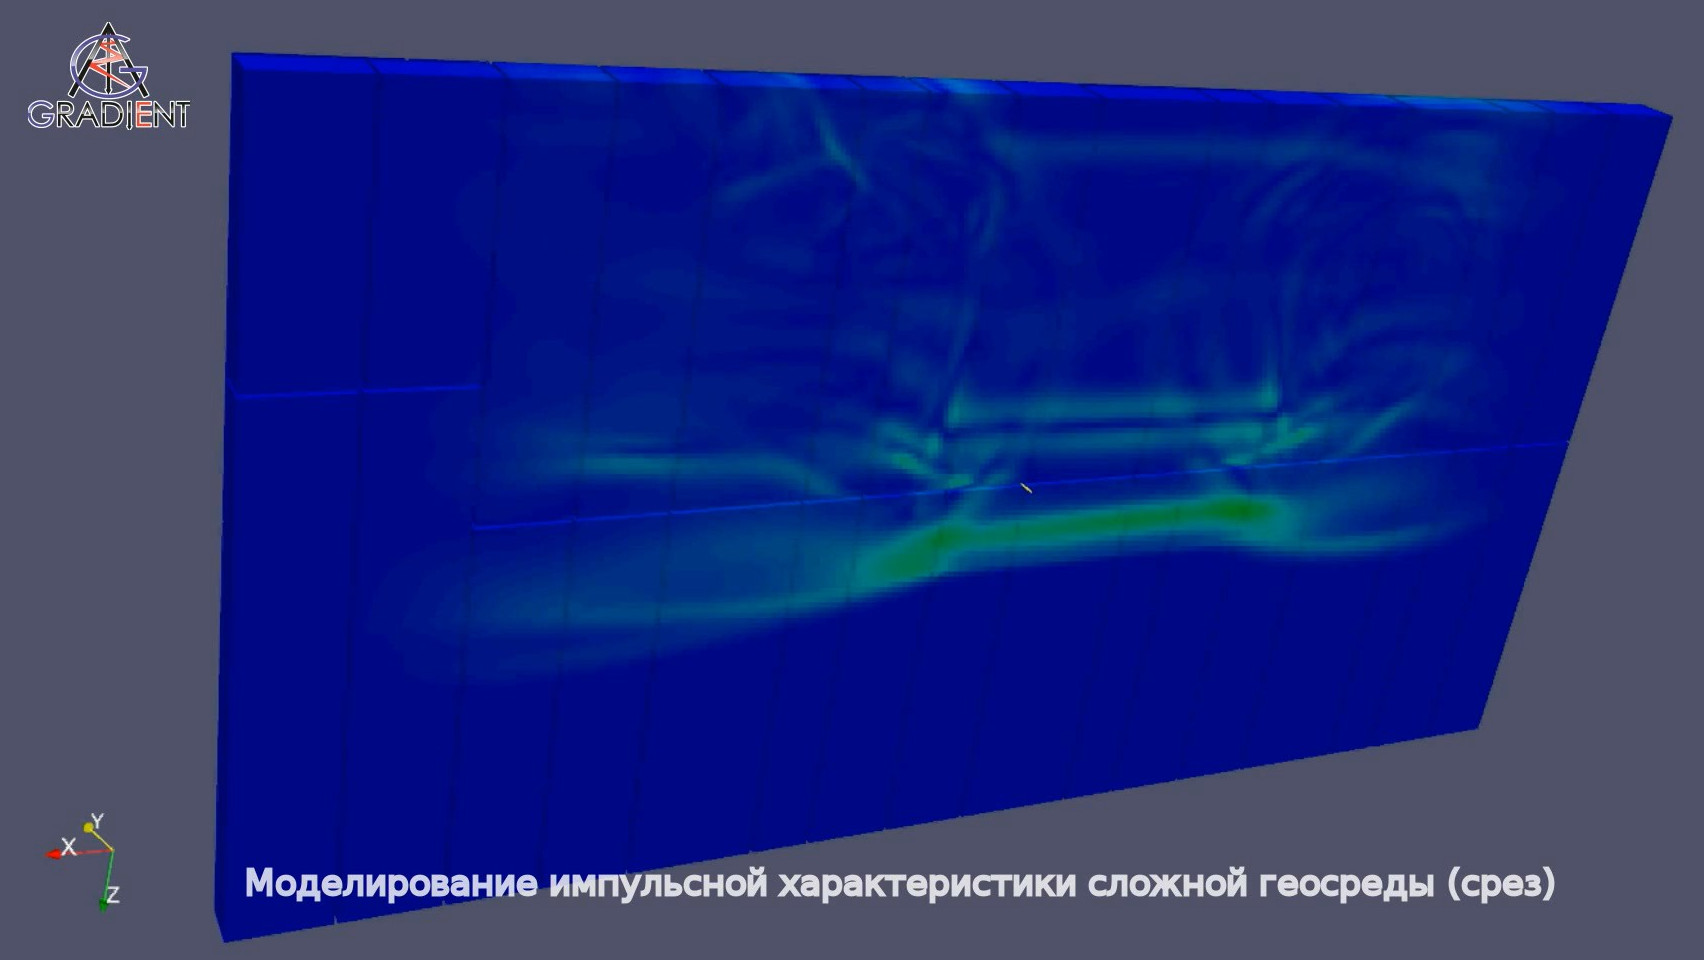
\includegraphics[width=\textwidth]{microseism}
            \end{figure}
        \end{column}
    \end{columns}
\end{frame}

\begin{frame}{Boost.odeint~--- библиотека численного интегрирования ОДУ}
    \begin{columns}
        \begin{column}{0.65\textwidth}
            \begin{itemize}
                \item Позволяет эффективно проводить параметрические
                    исследования ОДУ на GPU с помощью VexCL.
                \item[{[1]}] D. Demidov, K. Ahnert, K. Rupp, and P. Gottschling.\\
                    Programming CUDA and OpenCL: A Case Study Using Modern \CXX Libraries.\\
                    \emph{SIAM J. Sci. Comput.,} 35(5):C453 – C472, 2013.\\
                    \href{http://dx.doi.org/10.1137/120903683}{doi:10.1137/120903683}
                \item[{[2]}] K. Ahnert, D. Demidov, and M. Mulansky.\\
                    Solving ordinary differential equations on GPUs.\\
                    In \emph{Numerical Computations with GPUs} (pp. 125-157).  Springer, 2014.
                    \href{http://dx.doi.org/10.1007/978-3-319-06548-9\_7}{doi:10.1007/978-3-319-06548-9\_7}
            \end{itemize}
        \end{column}
        \begin{column}{0.35\textwidth}
            \begin{figure}
                \includegraphics[height=0.8\textheight]{ncwg}
            \end{figure}
        \end{column}
    \end{columns}
\end{frame}

\begin{frame}{Antioch}{A New Templated Implementation Of Chemistry for Hydrodynamics}
    \begin{columns}
        \begin{column}{0.5\textwidth}
            \begin{itemize}
                \item University of Texas at Austin, USA
                \item \www{https://github.com/libantioch/antioch}
                \item Гидродинамические расчеты с учетом химических реакций
                \item Для расчетов на GPU используется VexCL
            \end{itemize}
        \end{column}
        \begin{column}{0.5\textwidth}
            \begin{figure}
                \only<1>{
\includegraphics[width=\textwidth]{antioch-1}}%
                \only<2>{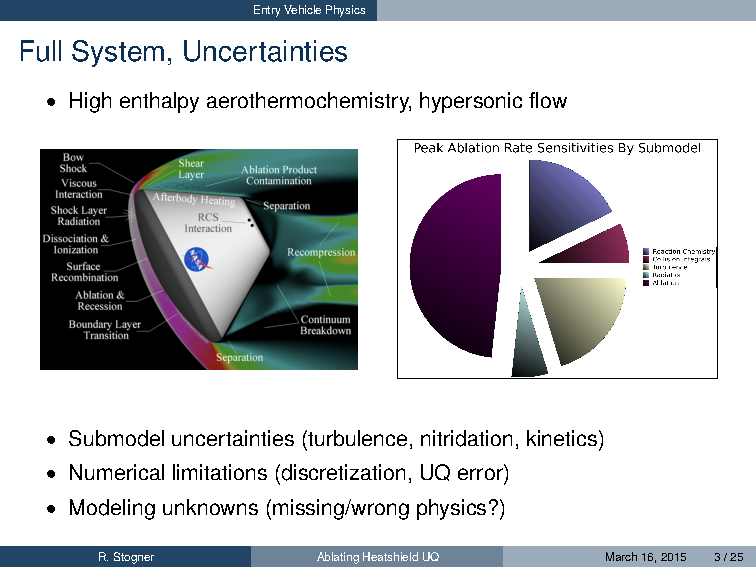
\includegraphics[width=\textwidth]{antioch-2}}
            \end{figure}
        \end{column}
    \end{columns}
\end{frame}

\begin{frame}{FDBB}{Fluid Dynamics Building Blocks}
    \begin{columns}
        \begin{column}{0.5\textwidth}
            \begin{itemize}
                \item Delft University of Technology, Netherlands
                \item \www{https://gitlab.com/mmoelle1/FDBB}
                \item Библиотека алгоритмов для вычислительной гидродинамики
                \item VexCL поддерживается как один из возможных бакендов
            \end{itemize}
        \end{column}
        \begin{column}{0.5\textwidth}
            \begin{figure}
                \includegraphics[width=\textwidth]{fdbb}
            \end{figure}
        \end{column}
    \end{columns}
\end{frame}



\begin{frame}{Шумоподавляющие фильтры для растровых изображений}
    \begin{columns}
        \begin{column}{0.4\textwidth}
            \begin{itemize}
                \item Pascal Schmitt, Georg-Augustus-Universit\"at,
                    G\"ottingen, Germany
                \item Ускорение~--- до 20x по сравнению с CPU
                \item Реализовал преобразование Фурье и генерацию случайных
                    чисел в VexCL
            \end{itemize}
        \end{column}
        \begin{column}{0.55\textwidth}
            \vspace{-1\baselineskip}
            \begin{figure}
                \only<1>{\includegraphics[height=\textheight]{neapel-1}}%
                \only<2>{\includegraphics[height=\textheight]{neapel-2}}
            \end{figure}
        \end{column}
    \end{columns}
\end{frame}

\begin{frame}{Оценка положения судна в пространстве}
    \begin{columns}
        \begin{column}{0.5\textwidth}
            \vspace{-2\baselineskip}
            \begin{figure}
                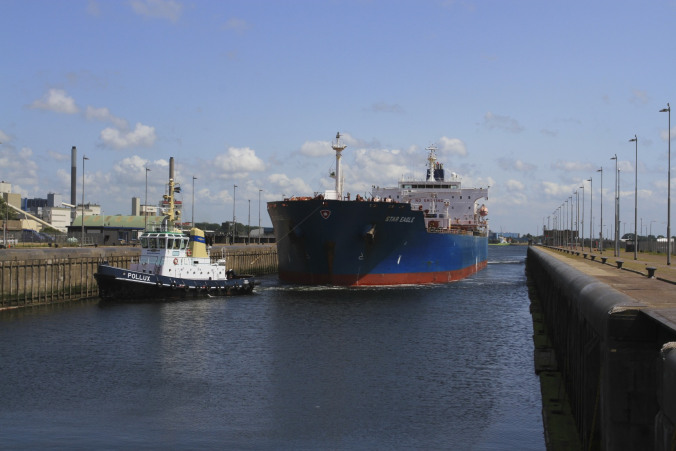
\includegraphics[width=0.8\textwidth]{ship-channel}
            \end{figure}
            \begin{itemize}
                \item University of Antwerp, Belgium
                \item Обработка данных лидара в реальном времени с помощью GPU
                \item Ускорение~--- 1000x по сравнению с примитивным алгоритмом
                    на CPU
            \end{itemize}
        \end{column}
        \begin{column}{0.45\textwidth}
            \vspace{-3\baselineskip}
            \begin{figure}
                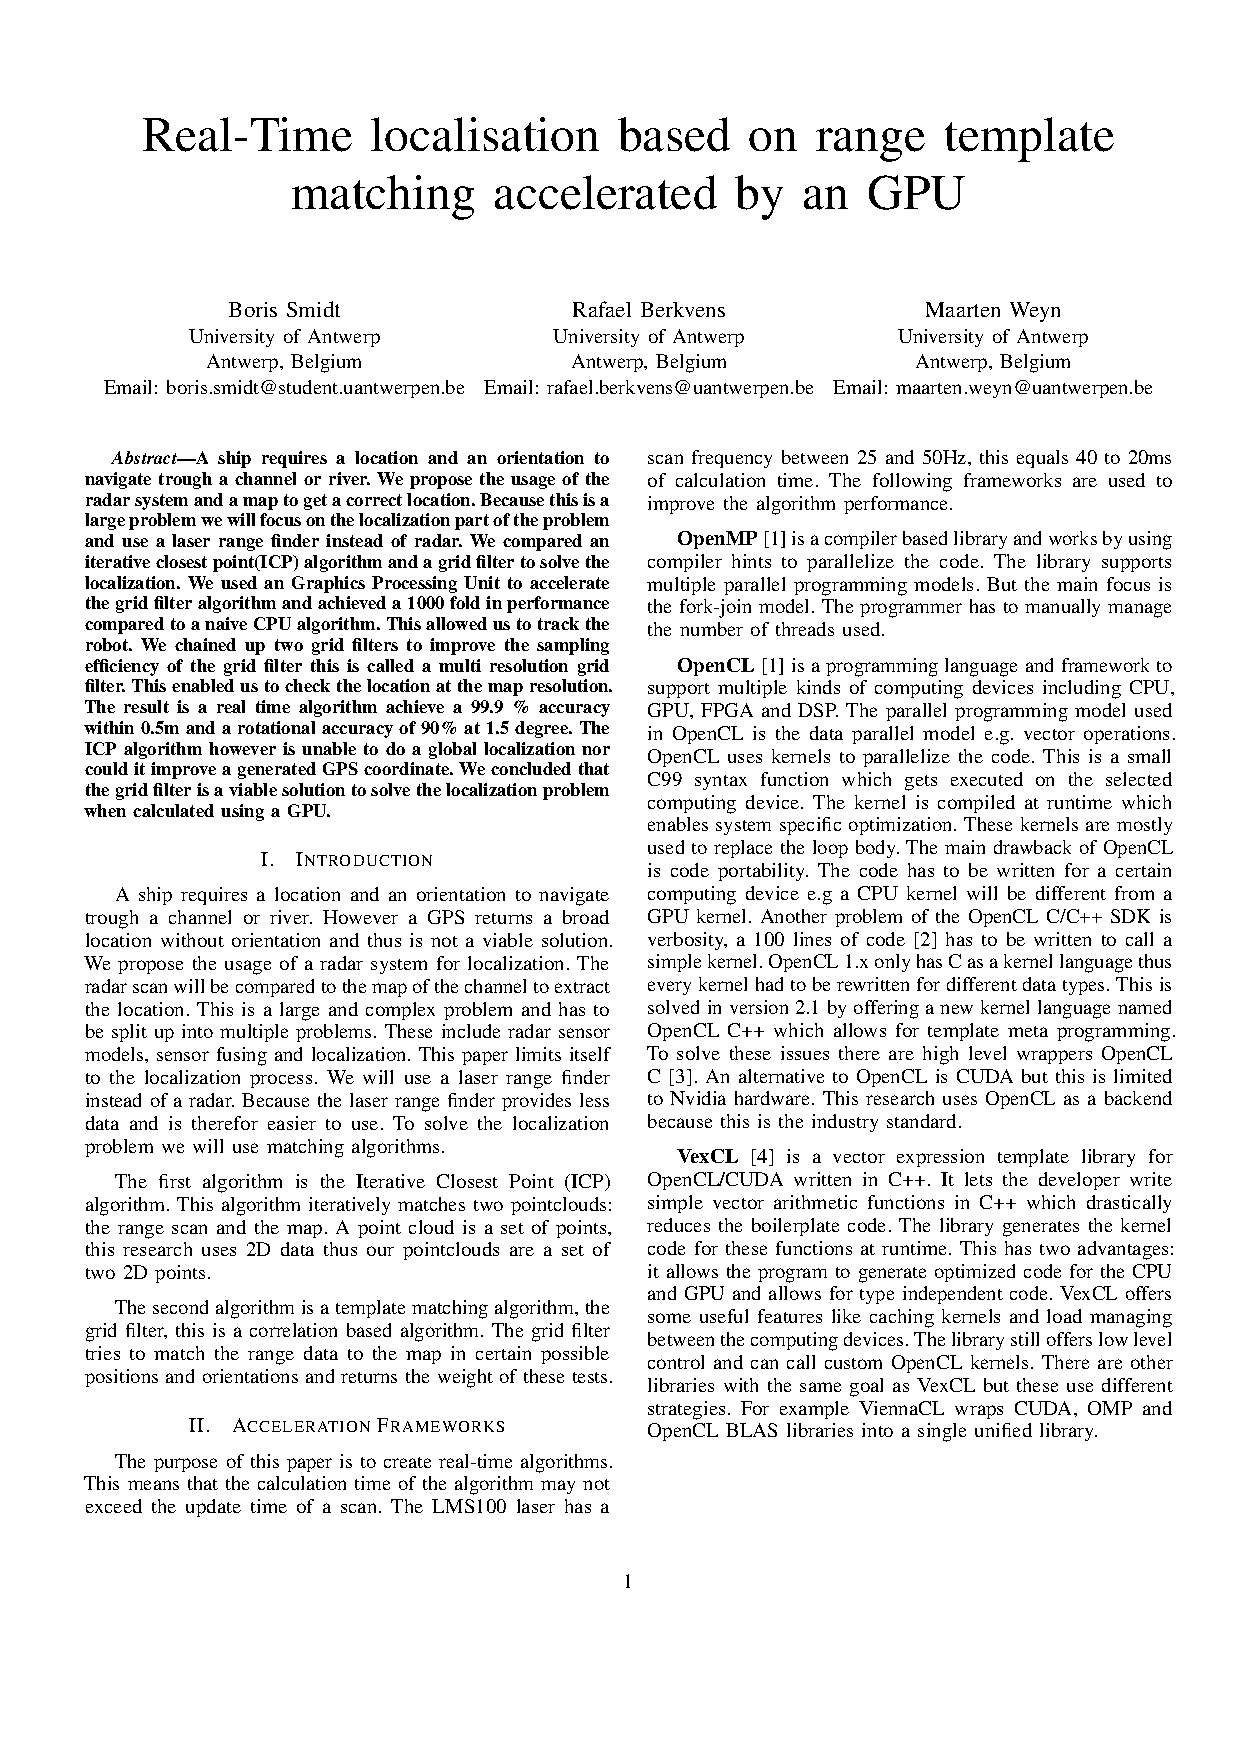
\includegraphics[height=1.05\textheight]{smidt}
            \end{figure}
        \end{column}
    \end{columns}
\end{frame}

\begin{frame}{AMGCL --- решение разреженных СЛАУ большой размерности}
    \forkme
    \begin{itemize}
        \item \www{https://github.com/ddemidov/amgcl}
        \item Реализация алгебраического многосеточного метода.
            \vspace{\baselineskip}
        \item Поддерживает несколько вычислительных бакендов:
            \begin{itemize}
                \item VexCL, CUDA, ViennaCL, OpenMP, \ldots
            \end{itemize}
        \item Позволяет использовать пользовательские типы и операции.
            \vspace{\baselineskip}
        \item Исходный код доступен под лицензией MIT
    \end{itemize}
\end{frame}

\begin{frame}{Kratos Multi-Physics}
    \begin{columns}
        \begin{column}{0.45\textwidth}
            \begin{itemize}
                \item International Center for Numerical Methods in
                    Engineering, Barcelona, Spain
                \item \www{http://www.cimne.com/kratos/}
                \item Пакет с открытым исходным кодом для инженерных расчетов
                \item В качестве решателя по умолчанию используется AMGCL
            \end{itemize}
        \end{column}
        \begin{column}{0.55\textwidth}
            \begin{figure}
                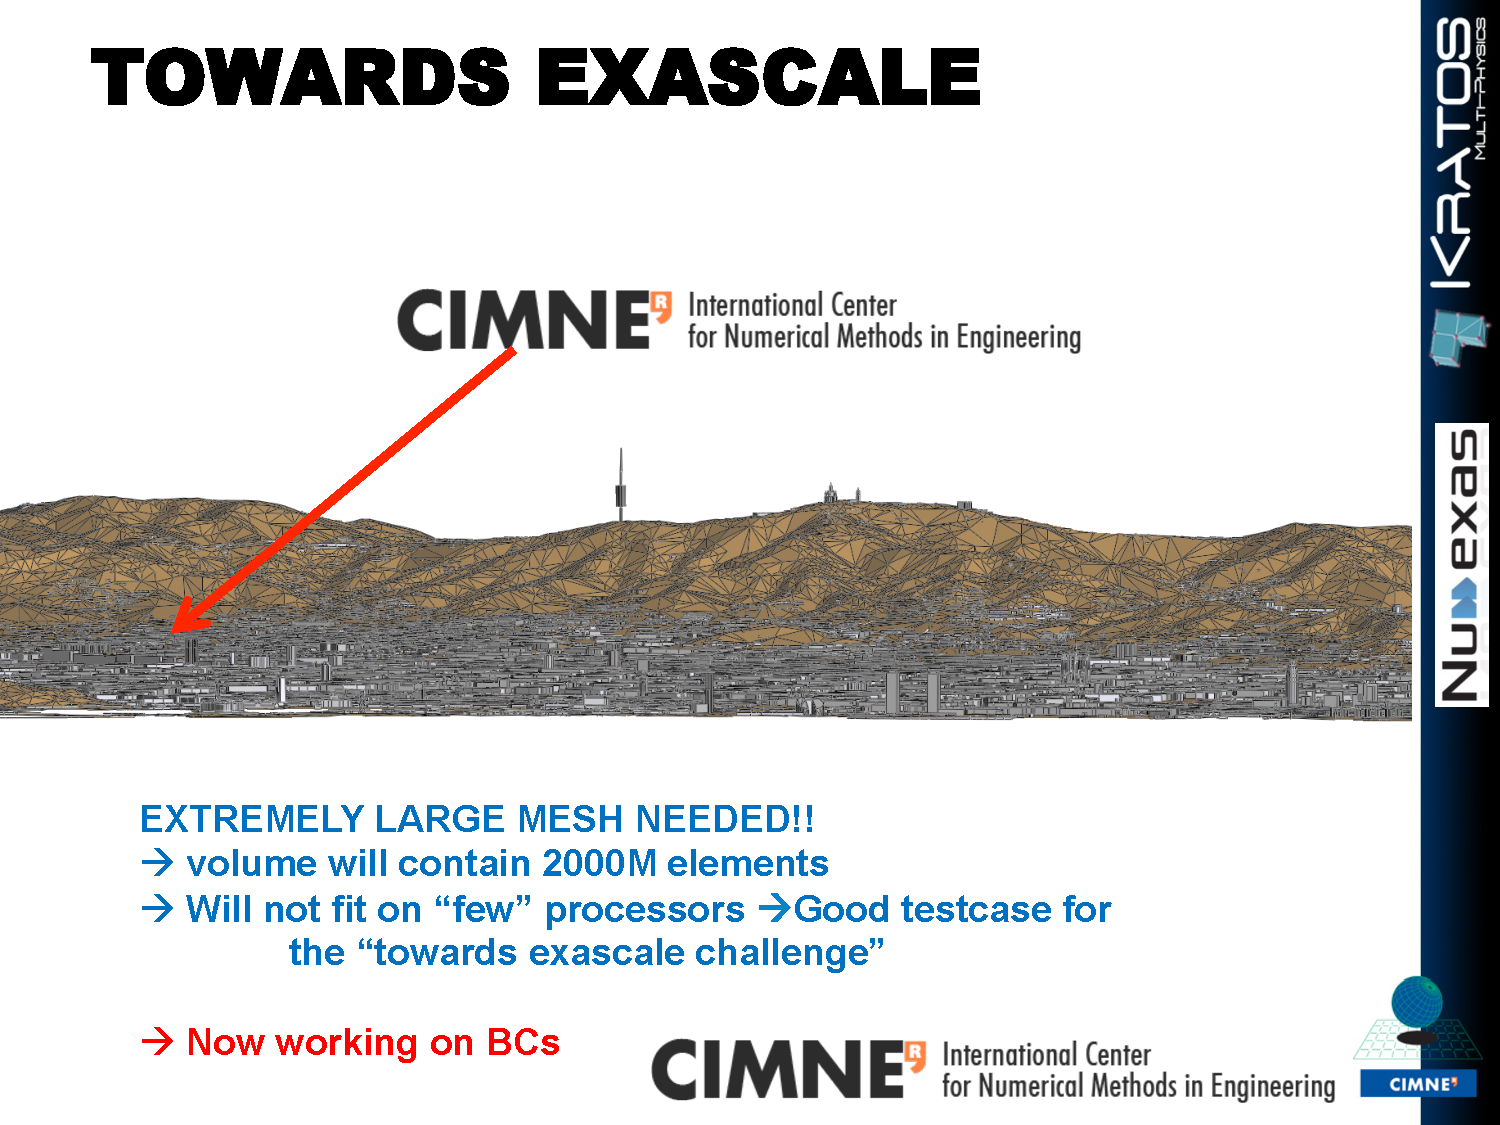
\includegraphics[width=\textwidth]{kratos}
            \end{figure}
        \end{column}
    \end{columns}
\end{frame}

%----------------------------------------------------------------------------
\begin{frame}{}
    \begin{itemize}
        \item Исходный код:
            \begin{itemize}
                \item \www{https://github.com/ddemidov/vexcl}
            \end{itemize}
            \vspace{\baselineskip}
        \item Документация:
            \begin{itemize}
                \item \www{http://vexcl.readthedocs.io}
            \end{itemize}
            \vspace{\baselineskip}
        \item Слайды:
            \begin{itemize}
                \item \www{https://speakerdeck.com/ddemidov}
            \end{itemize}
    \end{itemize}
\end{frame}

\end{document}
